\PassOptionsToPackage{unicode}{hyperref}
\documentclass[aspectratio=1610, 9pt]{beamer}

% Load packages you need here
%\usepackage{polyglossia}
%\setmainlanguage{german}

\usepackage{csquotes}

\usepackage{amsmath}
\usepackage{amssymb}
\usepackage{mathtools}

\usepackage{braket}
\usepackage{graphicx}

\usepackage{hyperref}
\hypersetup{
  linkcolor= {tudark}, % internal links
  citecolor={tugreen}, % citations
  urlcolor={tudark} % external links/urls
  }
\usepackage{bookmark}

\usepackage[english]{babel}
\usepackage[
backend=biber,
style=authoryear-comp
]{biblatex}

\bibliography{lit.bib}

\usepackage{siunitx}
\usepackage{multicol}

\usepackage{booktabs}

\definecolor{light-gray}{HTML}{b0b5b0}

% load the theme after all packages

\usetheme[
  showtotalframes, % show total number of frames in the footline
]{tudo}

% Put settings here, like
\unimathsetup{
  math-style=ISO,
  bold-style=ISO,
  nabla=upright,
  partial=upright,
  mathrm=sym,
}

\title{Classification und image-to-image transitioning anhand von Tiergesichtern}
\author[T.~Magorsch,~J.~L.~Späh]{Tom Magorsch\\ Jan Lukas Späh}
\institute[ML-Seminar]{\\[0.3cm]TU Dortmund \\ \Large ML-Seminar}

\begin{document}



\maketitle




\begin{frame}{Fragestellung}
\begin{itemize}
\item Verschiedene Fragestellungen:
\begin{enumerate}
\item Klassifikation: ``Befindet sich auf dem Bild ein Hund, eine Katze oder etwas anderes?''
\item Image-to-image Problem: ``Generiere ein Bild von einem Hund, einer Katze oder einem anderen Wildtier.''
\end{enumerate}
\item Weitere möglichen Untersuchungsschwerpunkte:
  \begin{itemize}
  \item Clustering von Arten und Rassen
  \item Data Augmentation von Trainings-Samples
  \end{itemize}
\end{itemize}



\end{frame}


\begin{frame}{Datensatz}
  \begin{columns}

    \column{0.8\textwidth}

    \begin{itemize}
    \item Quelle: \href{https://www.kaggle.com/andrewmvd/animal-faces?}{Kaggle}, Datensatz aus April 2020 (\href{https://arxiv.org/abs/1912.01865}{arxiv:1912.01865}) mit \href{https://github.com/clovaai/stargan-v2}{Git-Repo}
    \item Lizenz: CreativeCommons (CC BY-NC 4.0)
    \item Knapp $1600$ Bilder verschiedener Tiere: $512\times 512$ Pixel
    \item Bilder in drei Kategorien aufgeteilt: (jeweils ca. 5000 Bilder)
      \begin{enumerate}
      \item Cat
      \item Dog
      \item Wildlife
      \end{enumerate}
    \item Targetvariable im ersten Schritt: Prediction für jede Klasse
    \end{itemize}

    \column{0.2\textwidth}
    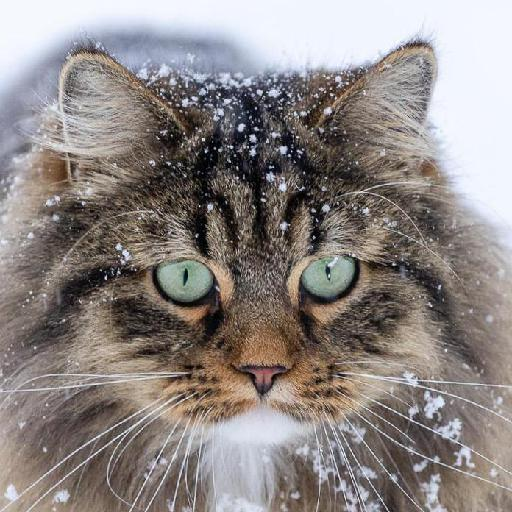
\includegraphics[scale=0.13]{images/cat.jpg}\\
    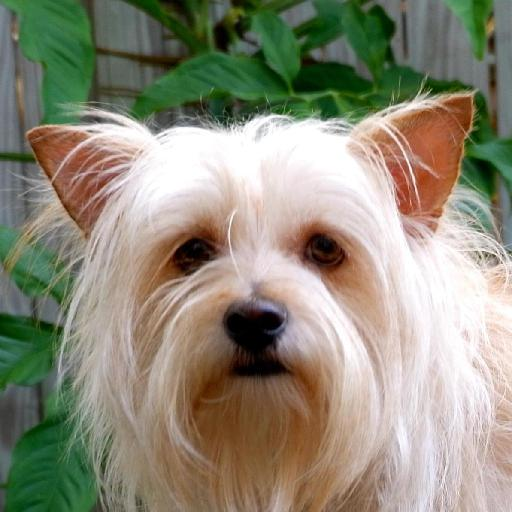
\includegraphics[scale=0.13]{images/dog.jpg}\\
    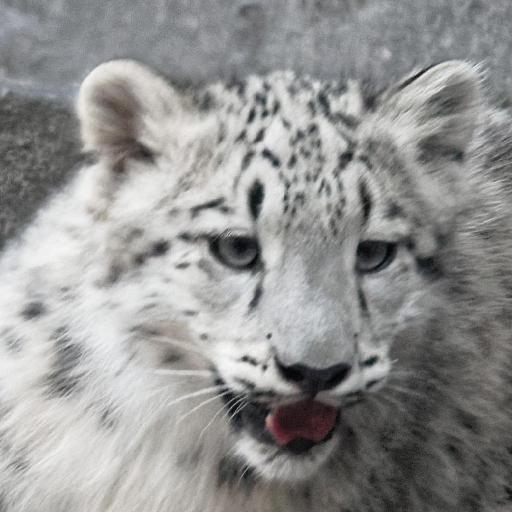
\includegraphics[scale=0.13]{images/wildlife.jpg}\\

  \end{columns}
\end{frame}

\begin{frame}{Vergleich mit Alternativmethode}
  \begin{itemize}
  \item Einfache Algorithmen sind kaum in der Lage, Bilder mit vergleichbarer Genauigkeit wie Deep-Learning-Methoden zu klassifizieren
  \item Mögliche Vergleichsmethode für image-classification: z.B. kNN:
  \begin{enumerate}
    \item Extrahiere Features manuell aus den Bilder (z. B. Farbhistogram, Kontrast, Form-Features)
    \item Definiere Metrik über dem Feature-Raum
    \item Nutze Metrik für klassischen kNN
  \end{enumerate}
  \item Performance Measure für GAN: Kann ein DNN die generierten von den echten Bildern unterscheiden ?
  \end{itemize}

\end{frame}



\end{document}
